\documentclass{ximera}

\title{Triple Integrals}
\author{Zack Reed}

\begin{document}
\begin{abstract}
In this activity we extend double integrals to three dimensions, exploring triple integrals for volume and mass calculations, along with cylindrical and spherical coordinate systems that simplify integration over curved 3D regions.
\end{abstract}
\maketitle

\section*{Introduction: From Double to Triple Integrals}

% APPLETS FOR REFERENCE

% https://www.geogebra.org/m/bqqfyjdm
% https://www.geogebra.org/m/sebfhwzx
% https://www.geogebra.org/m/xqrs44yg
% https://www.geogebra.org/m/hv9rk7hj
% https://www.geogebra.org/m/sgevexqr
% https://www.geogebra.org/m/yukegeqk
% https://www.geogebra.org/m/rwjghwbb

Just as we extended single integrals (summing over intervals) to double integrals (summing over 2D regions), we now extend to \textbf{triple integrals} that sum over 3D volumes.

\begin{problem}
Complete the pattern:
\begin{itemize}
    \item Single integral: $\displaystyle\int_a^b f(x)\,dx$ sums over a \wordChoice{\choice[correct]{1D interval}\choice{2D region}\choice{3D volume}}
    \item Double integral: $\displaystyle\iint_R f(x,y)\,dA$ sums over a \wordChoice{\choice{1D interval}\choice[correct]{2D region}\choice{3D volume}}
    \item Triple integral: $\displaystyle\iiint_E f(x,y,z)\,dV$ sums over a \wordChoice{\choice{1D interval}\choice{2D region}\choice[correct]{3D volume}}
\end{itemize}

What changes at each level?
\begin{selectAll}
    \choice[correct]{The dimension of the domain}
    \choice[correct]{The number of differentials}
    \choice{The fundamental idea of summing small pieces}
    \choice[correct]{The complexity of setting up bounds}
\end{selectAll}

\begin{feedback}
The core concept remains: integrals sum infinitesimal pieces. We're just extending to higher dimensions!
\end{feedback}
\end{problem}

\section*{The Challenge of Visualization}


An important limitation of triple integrals is that we \textbf{cannot easily visualize} the output of $f(x,y,z)$. Moreover, when we increase the input space to $4$ or more dimensions, we also lose the ability to visualize the input domain.

This limitation is why it's important to maintain the big idea, ``adding up pieces''. With all integral problems you figure out how to state the quantity you desire $M$ as a sum of small pieces $dM$. 

For triple integrals, we'll use the idea of ``mass'', $M$ as our physical intuition. 

Think of function being integrated as a density, and we're varying that density along a volume to get a total mass $M$ from small masses $dM$. Each small mass $dM$ will typically involve a product $\rho$ (the density function) with some differential element $dV$, and it's up to you to decide into how many dimensions you want to split $dV$ and how you accurately structure the sum accordingly.


\section*{Mass Integrals with Variable Density}

Because we lose the ability to use ``height'' as a visual metaphor for the contribution of the functions $f$ to the overall quantity $dM$, we need to switch to a new physical interpretation of how $f$ contributes to the integral.

This metaphor can carry into higher dimensions, even when we lose any kind of visual representation.

Think of the domain as a 3D object. We don't care just about how much space it takes up (volume), we also care how much ``stuff'' is in the object. This is its \textbf{mass}, as we've discussed before.

Below is a simple visual of a block in 3D space. We're going to use color as a stand in for density, where lighter greener colors represent less dense regions and darker blue-black colors represent more dense regions. The small cube represents a tiny volume element $dV$ that we will use to build up the mass of the object.


\begin{expandable}{stuff}{GeoGebra Instructions}
    Drag the point $(x,y,z)$ or use sliders to move the small volume element $dV$ around. The color represents density: brighter = less dense, darker = more dense.
\end{expandable}

\begin{center}
\geogebra{yn6dgycn}{740}{481}
\end{center}

\begin{problem}

Remember from prior sections that the basic model for mass is:

$$\text{mass}= \text{density} \times \text{volume}$$

This only applies when there is a constant density, however, so we need to use integrals to add up small density piecs $dM$ across the volume of the object.

Vary $x,y,z$ in the applet and choose the correct statements from below (select all that apply):

\begin{selectAll}
    \choice[correct]{The density $\rho$ is least at the bottom center of the cube}
    \choice{The density $\rho$ is least at the top right of the cube}
    \choice[correct]{The density is greatest on the corners of the cube}
    \choice{The density is greatest on the inside of the cube}
    \choice[correct]{The density $\rho$ increases as you move away from the origin $(0,0,0)$}
    \choice[correct]{The density $\rho$ increases as you increase $x$, $y$, and $z$}
    \choice{The density $\rho$ is greatest along the left side of the cube}
    \choice{The density $\rho$ is greatest along the right side of the cube}
\end{selectAll}

If density $\rho(x,y,z)$ varies throughout a 3D object, the small mass measurement is:
$$dM = \rho \cdot dV$$

The total mass adds up all of the tiny mass pieces:
$$M = \iiint_E dM = \iiint_E \rho\cdot \,dV$$

The $\iiint_E$ is just notation for ``adding up pieces along a 3D region $E$''. In this case, the region is a cube.

The cube is made from the box $-1 \leq x \leq 1$, $-1 \leq y \leq 1$, $0 \leq z \leq 2$. 

Select all of the correct comparisons of integrals. Remember that the bounds of integration together will form some rectangular region.

\begin{selectAll}
    \choice[correct]{$\displaystyle\int_{0}^1 \int_{0}^1 \int_1^2 \rho\,dz\,dy\,dx$ is greater than $\displaystyle\int_{-1}^0 \int_{-1}^0 \int_0^1 \rho\,dz\,dy\,dx$}
    \choice{$\displaystyle\int_{-1}^1 \int_{-1}^0 \int_0^2 \rho\,dz\,dy\,dx$ is greater than $\displaystyle\int_{-1}^1 \int_{0}^1 \int_0^2 \rho\,dz\,dy\,dx$}
    % more comparisons of this type, understanding a radial density function
    \choice[correct]{$\displaystyle\int_{.5}^1 \int_{.5}^1 \int_0^2 \rho\,dz\,dy\,dx$ is greater than $\displaystyle\int_{0}^{.5} \int_{0}^{.5} \int_0^2 \rho\,dz\,dy\,dx$}
    \choice{$\displaystyle\int_{0}^{.5} \int_{0}^{.5} \int_0^2 \rho\,dz\,dy\,dx$ is greater than $\displaystyle\int_{.5}^1 \int_{.5}^1 \int_0^2 \rho\,dz\,dy\,dx$}
    %an incorrect option
    % \choice{$\displaystyle\int_{-1}^1 \int_{-1}^1 \int_0^2 \rho\,dz\,dy\,dx$ is greater than $\displaystyle\int_{-1}^1 \int_{-1}^1 \int_0^2 \rho\,dz\,dy\,dx$}
\end{selectAll}
    
%some feedback
\begin{feedback}
The density is lowest at the origin and increases as you move away from it. The corners of the cube are the farthest from the origin, so they have the greatest density. Integrals with bounds that are farther from the origin will have greater mass because they include more of the higher density regions.
\end{feedback}
\end{problem}

Now that we have an intuition for how to interpret the integral $\displaystyle\iiint_E \rho\,dV$ as a sum of small mass pieces, we can start to compute some triple integrals.

The key difficulty in setting up these integrals is determining how to structure and order the bounds of integration in these complex volumes. That's what we'll practice next!


\section*{Setting up Triple Integrals}

For triple integrals, we have three variables $x,y,z$ and we integrate with respect to each, iteratively. Like with double integrals, we need to do some work up front to figure out the bounds of integration and the order of integration.

Start with a simple example and then we'll increase the complexity.

\begin{problem}
Compute the mass of the rectangular box $0 \leq x \leq 2$, $0 \leq y \leq 3$, $0 \leq z \leq 4$ with constant density $\rho(x,y,z) = 2$ kg/m³.

$$M = \int_0^2\int_0^3\int_0^4 2\,dz\,dy\,dx$$

\textbf{Innermost integral:}
$$\int_0^4 2\,dz = 2[z]_0^4 = \answer{8}$$

\textbf{Middle integral:}
$$\int_0^3 \int_0^4 2\,dz\,dy = 8[y]_0^3 = \answer{24}$$

\textbf{Outer integral:}
$$\int_0^2 \int_0^3 \int_0^4 2\,dz\,dy\,dx = 24[x]_0^2 = \answer{48}$$

In this case, because we have a constant density, we can check our work with the basic model of mass: $\rho \times V = 2 \times (2 \times 3 \times 4)=\answer{48}$ kg.

\begin{feedback}
For rectangular boxes with constant density, mass = density $\times$ volume! The triple integral naturally factors: $\rho \cdot \text{length} \times \text{width} \times \text{height}$.
\end{feedback}
\end{problem}

Now let's try a more complex example with a non-rectangular region and a variable density function.


\begin{problem}

Let's integrate the function $e^{z}$ over the wedge given in the first octant (where $x,y,z \geq 0$) and below the plane $x+y+z=1$.

We're interpreting this as if the density $\rho$ at each point $(x,y,z)$ is $e^{z}$, and we want to find the total mass of this wedge-shaped object.

\begin{center}
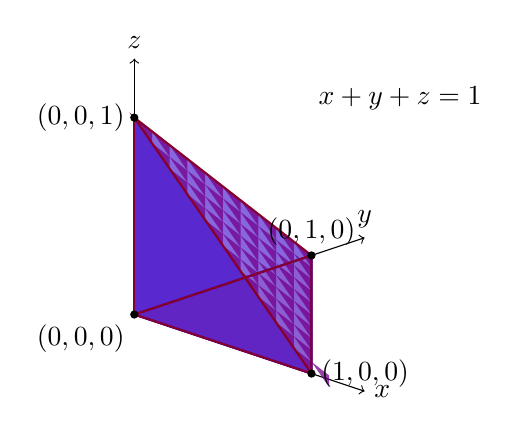
\begin{tikzpicture}[x={(0.9cm,-0.3cm)}, y={(0.9cm,0.3cm)}, z={(0cm,1cm)}, scale=2.5]
    % Draw axes
    \draw[->] (0,0,0) -- (1.3,0,0) node[right] {$x$};
    \draw[->] (0,0,0) -- (0,1.3,0) node[above] {$y$};
    \draw[->] (0,0,0) -- (0,0,1.3) node[above] {$z$};
    
    % Draw the triangular base in xy-plane
    \fill[blue!20, opacity=0.4] (0,0,0) -- (1,0,0) -- (0,1,0) -- cycle;
    \draw[thick, blue] (0,0,0) -- (1,0,0) -- (0,1,0) -- cycle;
    
    % Fill the three side walls
    \fill[purple!30!blue, opacity=0.6] (0,0,0) -- (1,0,0) -- (0,0,1) -- cycle;
    \fill[purple!30!blue, opacity=0.6] (0,0,0) -- (0,1,0) -- (0,0,1) -- cycle;
    \fill[purple!40!blue, opacity=0.6] (0,0,0) -- (1,0,0) -- (0,1,0) -- cycle;
    
    % Fill the top surface with colored triangular mesh
    \foreach \i in {0,1,...,9} {
        \foreach \j in {0,1,...,\i} {
            \pgfmathsetmacro{\xa}{(10-\i)/10}
            \pgfmathsetmacro{\ya}{\j/10}
            \pgfmathsetmacro{\xb}{(10-\i-1)/10}
            \pgfmathsetmacro{\yb}{\j/10}
            \pgfmathsetmacro{\yc}{(\j+1)/10}
            \pgfmathsetmacro{\za}{1-\xa-\ya}
            \pgfmathsetmacro{\zb}{1-\xb-\yb}
            \pgfmathsetmacro{\zc}{1-\xb-\yc}
            \fill[purple!60!blue, opacity=0.75] 
                (\xa,\ya,\za) -- (\xb,\yb,\zb) -- (\xb,\yc,\zc) -- cycle;
        }
    }
    
    % Draw boundary edges of the slanted face
    \draw[thick, purple!70!black] (1,0,0) -- (0,1,0) -- (0,0,1) -- cycle;
    
    % Draw outline edges
    \draw[thick, purple!70!black] (0,0,1) -- (0,0,0);
    \draw[thick, purple!70!black] (1,0,0) -- (0,0,0);
    \draw[thick, purple!70!black] (0,1,0) -- (0,0,0);
    
    % Label the plane
    \node at (.75,.75,1.1) {$x+y+z=1$};
    
    % Mark vertices
    \fill[black] (0,0,0) circle (0.6pt) node[below left] {$(0,0,0)$};
    \fill[black] (1,0,0) circle (0.6pt) node[right] {$(1,0,0)$};
    \fill[black] (0,1,0) circle (0.6pt) node[above] {$(0,1,0)$};
    \fill[black] (0,0,1) circle (0.6pt) node[left] {$(0,0,1)$};
\end{tikzpicture}
\end{center}

This wedge is bounded by:
\begin{itemize}
    \item The three coordinate planes: $x=\answer{0}$, $y=\answer{0}$, $z=\answer{0}$
    \item The slanted plane: $x+y+z=\answer{1}$
\end{itemize}

Before we worry about the function we're integrating, we need to set up the bounds of integration.

The differential volume element in rectangular coordinates is: $dV = \answer{dx} \cdot \answer{dy} \cdot \answer{dz}$ (ordered $x$ then $y$ then $z$).

This represents the volume of a tiny \wordChoice{\choice{sphere}\choice{cylinder}\choice[correct]{rectangular box}\choice{pyramid}}.

Let's set up the bounds for the wedge. 

The bounds of integration are essential a variable-by-variable description of the solid, but we have to keep track of what variables depend on each other.

\textbf{Step 1: Choose an order}

We'll integrate in the order $dz\,dy\,dx$. In many cases, the choice of order will make the integral easier or harder to compute (using the Fundamental Theorem of Calculus).

\textbf{Step 2: Find $z$ bounds}

As we integrate, we will ``lose'' one variable at a time, reducing the complexity of the bounds. We'll start with the first variable, in this case $z$.
For a fixed point $(x,y)$ in the $xy$-plane, $z$ ranges from the bottom ($z=0$) up to the slanted plane $z = 1 - x - y$.

So: $0 \leq z \leq \answer{1-x-y}$

\begin{center}
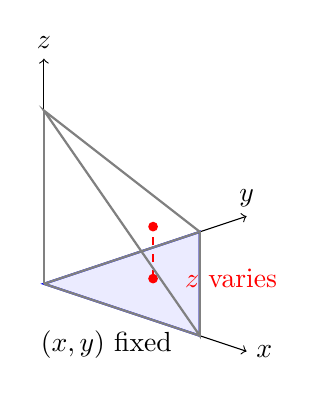
\begin{tikzpicture}[x={(0.9cm,-0.3cm)}, y={(0.9cm,0.3cm)}, z={(0cm,1cm)}, scale=2.2]
    \draw[->] (0,0,0) -- (1.3,0,0) node[right] {$x$};
    \draw[->] (0,0,0) -- (0,1.3,0) node[above] {$y$};
    \draw[->] (0,0,0) -- (0,0,1.3) node[above] {$z$};
    
    \fill[blue!20, opacity=0.4] (0,0,0) -- (1,0,0) -- (0,1,0) -- cycle;
    \draw[thick, blue] (0,0,0) -- (1,0,0) -- (0,1,0) -- cycle;
    
    % Show a vertical line at a fixed (x,y)
    \pgfmathsetmacro{\xa}{0.3}
    \pgfmathsetmacro{\ya}{0.4}
    \pgfmathsetmacro{\za}{1-\xa-\ya}
    \draw[thick, red, dashed] (\xa,\ya,0) -- (\xa,\ya,\za);
    \fill[red] (\xa,\ya,0) circle (0.8pt);
    \fill[red] (\xa,\ya,\za) circle (0.8pt);
    \node[red] at (\xa+0.5,\ya,\za/2) {$z$ varies};
    %below (0,0,0)
    \node at (.2,.2,-0.35) {$(x,y)$ fixed};
    
    % Draw the wedge outline
    \draw[thick, gray] (1,0,0) -- (0,1,0) -- (0,0,1) -- cycle;
    \draw[thick, gray] (0,0,1) -- (0,0,0);
    \draw[thick, gray] (1,0,0) -- (0,0,0);
    \draw[thick, gray] (0,1,0) -- (0,0,0);
\end{tikzpicture}
\end{center}

\textbf{Step 3: Find $y$ bounds}

Now we express the variation in $y$ within our region.

Looking down from above (into the $xy$-plane), the wedge looks like the triangle with vertices $(0,0)$, $(1,0)$, $(0,1)$.

For a fixed $x$ value, $y$ ranges from $0$ to the line connecting $(1,0)$ and $(0,1)$.

This line has equation $y = \answer{1-x}$.

So: $0 \leq y \leq \answer{1-x}$

\begin{center}
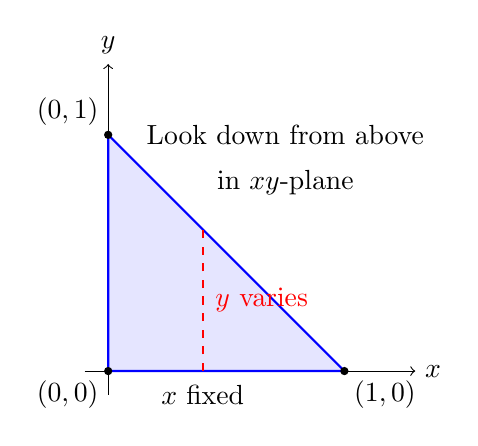
\begin{tikzpicture}[scale=3]
    \draw[->] (-0.1,0) -- (1.3,0) node[right] {$x$};
    \draw[->] (0,-0.1) -- (0,1.3) node[above] {$y$};
    
    % Fill the triangular projection
    \fill[blue!20, opacity=0.5] (0,0) -- (1,0) -- (0,1) -- cycle;
    \draw[thick, blue] (0,0) -- (1,0) -- (0,1) -- cycle;
    
    % Show a vertical slice at fixed x
    \pgfmathsetmacro{\xval}{0.4}
    \pgfmathsetmacro{\ymax}{1-\xval}
    \draw[thick, red, dashed] (\xval,0) -- (\xval,\ymax);
    \node[red] at (\xval+0.25,\ymax/2) {$y$ varies};
    \node at (\xval,-0.1) {$x$ fixed};
    
    % Mark vertices
    \fill[black] (0,0) circle (0.5pt) node[below left] {$(0,0)$};
    \fill[black] (1,0) circle (0.5pt) node[below right] {$(1,0)$};
    \fill[black] (0,1) circle (0.5pt) node[above left] {$(0,1)$};
    
    \node at (0.75,1) {Look down from above};
    \node at (0.75,.8) {in $xy$-plane};
\end{tikzpicture}
\end{center}

\textbf{Step 4: Find $x$ bounds}

Finally, $x$ ranges over the entire base: $0 \leq x \leq \answer{1}$

\textbf{Step 5: Write the integral}

Suppose this wedge has density function $\rho(x,y,z) = e^{z}$ (mass per unit volume increasing exponentially with height).

To find the total mass:
$$M = \iiint_E \rho(x,y,z)\,dV = \int_0^{\answer{1}} \int_0^{\answer{1-x}} \int_0^{\answer{1-x-y}} e^{z}\,dz\,dy\,dx$$

\textbf{Step 6: Compute the integral}

Let's evaluate this step by step.

\textbf{Inner integral}
$$\int_0^{1-x-y} e^{z}\,dz = \left[\answer{e^z}\right]_0^{1-x-y} = e^{1-x-y} - \answer{1}$$

\textbf{Middle integral}
$$\int_0^{1-x} (e^{1-x-y} - 1)\,dy = \int_0^{1-x} e^{1-x-y}\,dy - \int_0^{1-x} 1\,dy$$

For the first part, let $u = 1-x-y$, so $du = \answer{-dy}$ (with respect to $y$).
$$\int_0^{1-x} e^{1-x-y}\,dy = \int_{1-x}^0 e^{u} \, (-du) = \int_0^{1-x} e^{u} \, du = \left[\answer{e^u}\right]_0^{1-x} = \answer{e^{1-x} - 1}$$

For the second part:
$$\int_0^{1-x} 1\,dy = \answer{1-x}$$

Combining:
$$\int_0^{1-x} (e^{1-x-y} - 1)\,dy = (e^{1-x} - 1) - (1-x) = \answer{e^{1-x} - 2 + x}$$

\textbf{Outer integral}
$$M = \int_0^1 (e^{1-x} - 2 + x)\,dx$$

Evaluate each term:
$$\int_0^1 e^{1-x}\,dx = \left[\answer{-e^{1-x}}\right]_0^1 = -e^0 + e^1 = \answer{e - 1}$$

$$\int_0^1 (-2 + x)\,dx = \left[-2x + \frac{x^2}{2}\right]_0^1 = -2 + \frac{1}{2} = \answer{-3/2}$$

Therefore:
$$M = (e - 1) + \left(-\frac{3}{2}\right) = \answer{e - 5/2}$$
\end{problem}


\end{document}